\documentclass{standalone}
\usepackage{pgfplots}
\usepackage{amsmath}

\begin{document}

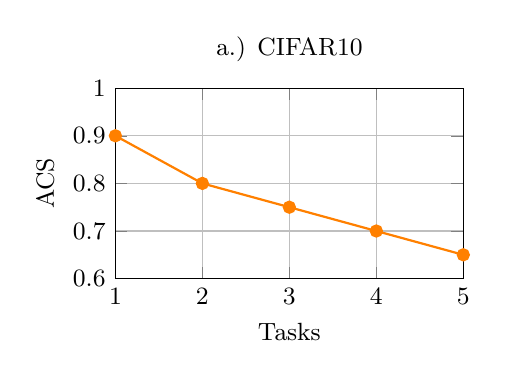
\begin{tikzpicture}
    \begin{axis}[
        width=6cm,
        height=4cm,
        grid=major,
        xmin=1, xmax=5,
        ymin=0.6, ymax=1.0,
        xlabel={Tasks},
        ylabel={ACS},
        title={a.) CIFAR10},
        title style={font=\small},
        label style={font=\small},
        tick label style={font=\small},
        every axis plot/.append style={thick, mark=*},
        legend pos=south west
    ]
    \addplot[color=orange, mark=*, mark options={fill=orange}] coordinates {
        (1,0.9) (2,0.8) (3,0.75) (4,0.7) (5,0.65)
    };
    \end{axis}
\end{tikzpicture}
\hspace{1cm}
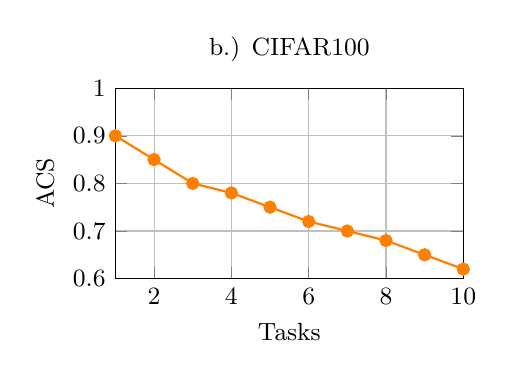
\begin{tikzpicture}
    \begin{axis}[
        width=6cm,
        height=4cm,
        grid=major,
        xmin=1, xmax=10,
        ymin=0.6, ymax=1.0,
        xlabel={Tasks},
        ylabel={ACS},
        title={b.) CIFAR100},
        title style={font=\small},
        label style={font=\small},
        tick label style={font=\small},
        every axis plot/.append style={thick, mark=*},
        legend pos=south west
    ]
    \addplot[color=orange, mark=*, mark options={fill=orange}] coordinates {
        (1,0.9) (2,0.85) (3,0.8) (4,0.78) (5,0.75) 
        (6,0.72) (7,0.7) (8,0.68) (9,0.65) (10,0.62)
    };
    \end{axis}
\end{tikzpicture}

\end{document}